\documentclass[a4paper,12pt]{article}

\usepackage{cmap}
\usepackage{mathtext}
\usepackage[T2A]{fontenc}
\usepackage[utf8]{inputenc}
\usepackage[english,russian]{babel}
\usepackage{listings}

\usepackage{amsmath,amsfonts,amssymb,amsthm,mathtools}
\usepackage{icomma}
\usepackage{upgreek}
\mathtoolsset{showonlyrefs=true}

\usepackage{tabto}
\usepackage{euscript}
\usepackage{mathrsfs}

\usepackage[top=3cm, bottom=1.5cm]{geometry}
\usepackage{graphicx}

\newcommand*{\hm}[1]{#1\nobreak\discretionary{}
{\hbox{$\mathsurround=0pt #1$}}{}}

\author{Kupriyanov Kirill}
\title{Data Analysis PI\\Theoretical assignment $\#6$}
\date{}

\begin{document}
\maketitle
\thispagestyle{empty}
\newpage
\section*{Task 1.}
\underline{\textit{Problem:}} Consider a linearly separable dataset and SVM
with polynomial kernel \(K(x, y) = (x^\top y + 1)^d\). Is that right, that for
any \(d > 1\) the decision boundary representation in initial feature space
will be the \textbf{error - free hyperplane} (linear decision boundary).\\
\newline
\underline{\textit{Solution:}} The decision boundary just cannot be linear if the
kernel is RBF and \(d > 1\).

For example,

\begin{figure}[h]
    \centering
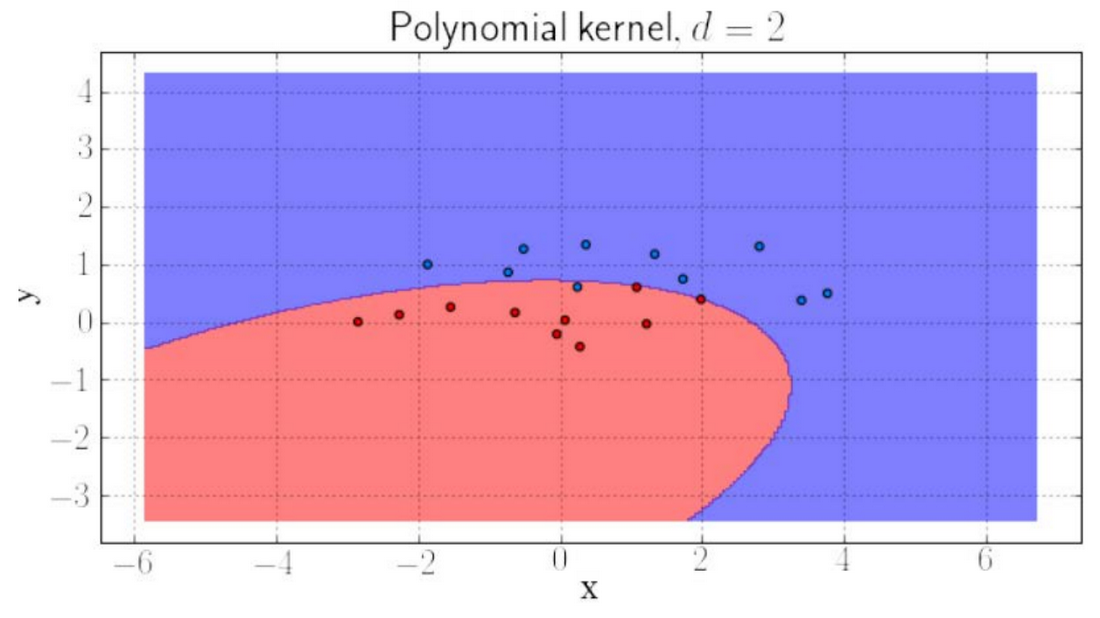
\includegraphics[width=0.7\textwidth]{example1}
\end{figure}

\newpage
\section*{Task 2.}
\underline{\textit{Problem:}} Find the computational complexity of the linear and kernel SVM \textbf{classification} procedure of a single
object (SVM is already trained).\\
\newline
\underline{\textit{Solution:}} If an input feature vector is a vector of float values, then the result is
\[
    Y = f(wx) = f\left(\sum\limits_{i=1}^{n}w_ix_i\right)
\]
Where \(w\) is a weight matrix, \(f\) - function to compute the result from dot
product.

So, the space complexity of classifying 1 object using a linear classifier
is equal to complexity of computing dot product of 2 vectors.
\[
    O(f) = O(d)
\]
,d - number of features.

SVC:
\[
    a(x) = sign(\sum\limits_{i=1}^{n} \lambda i\cdot ci\cdot xi\cdot x - b)
\]
Where:

\(x_i\) - a sample object.

\(x\) - a classidied object.

Using only those objects, for which \(\lambda \neq 0\), let's assume that \(m\) is number of objects for which \(\lambda \neq 0\). Then, the complexity will be \(O(md)\). d - number of features.

So, the linear classifier is \(O(d)\), and SVM is \(O(md)\)


\newpage
\section*{Task 3.}
\underline{\textit{Problem:}} Consider SVM regression optimization problem. Write down dual formulation of that problem with
Lagrangian and Karush-Kuhn-Takker theorem.\\
\newline
\underline{\textit{Solution:}} \(\varepsilon\) - insensitive error function

\[
    E_\varepsilon(a(x) - y)=
    \begin{cases}
        0 &\mbox{if } |a(x) - y| < \varepsilon \\
        |a(x) - y| - \varepsilon &\mbox{else} 
    \end{cases}
\]
The goal is to minimize a regularized error function given by
\[
    C\sum^l_{i=1}E_\varepsilon(a(x_i)-y_i)+\frac{1}{2C}||w||^2
\]
Let the slacks variables be:
\begin{gather}
    \xi^+_i = (\langle w,x_i \rangle - w_0 - y_i - \varepsilon)_+ \geqslant 0\\
    \xi^-_i = (-\langle w,x_i \rangle - w_0 + y_i - \varepsilon)_+ \geqslant 0
\end{gather}

SVR error function:
\[
    \frac{1}{2}||w||^2 + C\sum_{i=1}^l(\xi_i^++\xi_i^-) \rightarrow min_{w,w_0,\xi^+,\xi^-}
\]
The Lagrange multipliers are \(a_n\geqslant 0,\hat{a}_n \geqslant 0, \mu_n\geqslant0\) and \(\hat{\mu}\geqslant 0\)
\[
    L = C\sum_{i=1}^l(\xi_i^++\xi_i^-) + \frac12||w||^2 - \sum_{i=1}^l(\mu_i\xi_i^++\hat{\mu}\xi_i^-) - \sum_{i=1}^la_i(\varepsilon+\xi_i^++a_i-y_i) - \sum_{i=1}^l\hat{a_i}(\varepsilon+\xi_i^--a_i+y_i)
\]

\begin{gather}
    \frac{dL}{dw}=0 \rightarrow w = \sum_{i=1}^l(a_i-\hat{a}_i)x_i\\
    \frac{dL}{db}=0 \rightarrow \sum_{i=1}^l(a_i-\hat{a}_i) = 0\\
    \frac{dL}{d\xi_i^+}=0 \rightarrow a_i+\mu_i = C\\
    \frac{dL}{d\xi_i^-}=0 \rightarrow \hat{a}_i+\hat{\mu}_i = C\\
\end{gather}

So the dual problem:
\[
    L(a,\hat{a}) = -\frac12\sum_{i=1}^l\sum_{j=1}^l(a_i-\hat{a}_i)(a_j-\hat{a}_j)\varphi(x_i,x_j)-\varepsilon \sum_{i=1}^l(a_i+\hat{a}_i)+\sum_{i=1}^l(a_i-\hat{a}_i)y_i
\]

\end{document}


% EOF

